\chapter{Introduction}
\label{chap:introduction}

\section{Initial Situation}
Digital Twins (DT) are a key technology at the front of the fourth industrial revolution, coined Industry 4.0.
The latter term is characterized by the interaction of cyber-physical systems (CPS), the Internet of Things (IoT), and cloud computing to create smart factories with the goal of automation and efficiency \parencite{Oztemel2020}. Companies pursue this ideal by trying to remain competitive through the adoption of innovative technologies that promise enhanced productivity and reduced operational costs. One such technology that supports this transformation is the DT. It can be defined as a virtual representation of physical assets enabling real-time monitoring and optimization \parencite{Tao2018ijamt}. The DT bridges the connection between the two entities with a bi-directional data flow to exchange information and to influence the behaviour of the physical asset \parencite{grieves2014digital}. This technology in Industry 4.0 connects the physical and digital worlds through real-time data integration, simulation, and optimization \parencite{judijanto2024trends}.

Although this field is rapidly evolving, a unified definition of DT has yet to be established due to the diverse requirements and perspectives across different fields. In engineering, the focus might be on the real-time interaction between physical systems and their digital counterparts, whereas in computer science, the emphasis is often on data integration and simulation capabilities. These varying priorities result in multiple interpretations and applications of the term DT. The term was first introduced by Michael Grieves in 2002, defining it as a digital representation of a physical object or system \parencite{grieves2014digital}. However, the concept has evolved since then, encompassing a broader range of applications and technologies. Going back through the literature, there are three terms used to describe similar characteristics of DT: Digital Model (DM), Digital Shadow (DS), and Digital Twin (DT), see \Cref{fig:Kritzinger} \parencite{jones2020characterising,Zhang2021jmsy}.

\begin{figure}[htbp]
  \centering
  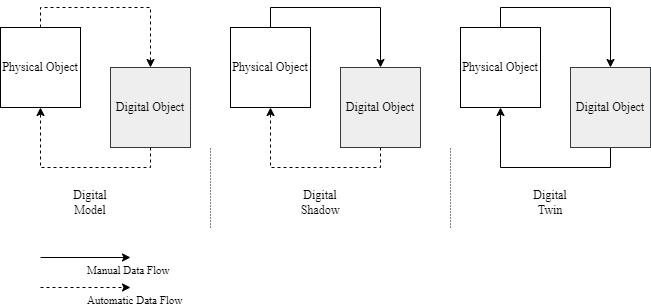
\includegraphics[width=0.8\textwidth]{figures/kritzinger.png}
  \caption{Comparison of Digital Shadow (DS), Digital Model (DM) and Digital Twin (DT) as presented by Kritzinger (2018). This distinction is crucial for understanding validation requirements across different digital representation types.}
  \label{fig:Kritzinger}
\end{figure}

The DM represents the most basic form. It contains manual data connections between physical and digital entities. These connections can be temporarily shifted or even disconnected. There is no control of the digital object over the physical entity. It rather is a simple or complex model \textit{describing} the modelled object. It can not make decisions by itself to influence the physical object. The reason lies in the potential outdated data the digital part possesses or in the fact that it does not contain logic to control the data flow back to the physical part by itself. The control and the obligation to interpret the results is completely in the hands of the modeller.
The DS is a more advanced version of the DM. It is a digital representation of the physical object, which is continuously updated with real-time data. The DS can be used for monitoring, analysis and simulation purposes. It can predict the future state of the physical object based on the current state and historical data. However, the DS is not able to influence the physical object. The control is, similar to the DM, still in the hands of the modeller. A DS is frequently used for simulation purposes and is often misclassified as a DT in the literature \parencite{kritzinger2018digital,buildings11040151}.
The DT is the most advanced version of the triplet. It is a digital representation of the physical object, which is also continuously updated with real-time data. The DT can be used for monitoring, analysis, and \textit{control} purposes. It can predict the future state of the physical object based on the current state and historical data. The DT can also influence the physical object by sending control signals to it. The control is partially or completely in the hands of the DT. The DT thus \textit{can} serve more purpose than modelling or simulating the physical object. It may serve as an autonomic system, updating itself or by help of the modeller \parencite{kritzinger2018digital}.

DTs are applied across various sectors, including manufacturing, defense, automotive, service, finance and healthcare \parencite{Tao2018ijamt}. Manufacturing stands out due to its high potential for process optimization and automation. This thesis focuses on the latter, particularly discrete material flow systems (DMFS). These systems process discrete objects (parts) that move along transportation routes or conveyor lines—either at regular or irregular intervals—integrating both production and logistics operations \parencite{arnold2005materialfluss, schwede2024learning}. A core simplification in their modeling is the abstraction of material flow as a sequence of discrete events, in accordance to the principles of discrete-event simulation (DES) \parencite{kovacs2016mathematical, robinson2014simulation}. DES is particularly well-suited for analyzing complex systems where state changes occur at discrete points in time, such as arrivals, departures, and processing steps \parencite{robinson2014simulation}.

In hindsight, DM played a crucial role in the design, planning, and control of DMFS, primarily through applications such as material flow simulations, logistic assistance systems, and digital factory implementations \parencite{Thiede2013}. However, advancements in both DS and DT have enabled a revolution from isolated, usecase-specific models toward complete digital representations that span the entire lifecycle of DMFS \parencite{Abdoune2023}. This transition is largely driven by the increasing demand for predictive capabilities by stakeholders and automated decision support in manufacturing systems, reflecting the cornerstones of Industry 4.0 \parencite{frank2019industry}. A second driver of DT innovation lies in the widely available data from IoT devices and sensors. Unlocking these potentials in model training and real-time adaption of the DT is crucial for its modelling capabilities \parencite{Tao2018ijamt}.

In practice, the automated data transfer between the digital model and the physical system is of secondary importance for DMFS management. Unlike in time-critical applications, human decision-makers remain an integral part of the control loop, ensuring that real-time automation is not always necessary \parencite{schwede2024learning}. Consequently, for this thesis, digital simulations and DTs will be treated as equivalent concepts.

Beyond merely replicating the current state and managing historical data, DTs serve a crucial function in predicting system behavior and evaluating potential modifications. The widespread adoption of DES within digital twins highlights the central role of simulation-based digital twins (SBDT) in DMFS \parencite{Lugaresi2021aifac}. As \citeauthor{schwede2024learning} emphasize, SBDTs provide decision support for optimizing cost and performance in highly competitive manufacturing environments. While current SBDTs are primarily developed and updated manually by domain experts, emerging research explores how machine learning (ML) can enhance predictive accuracy and automate model updates by automatically learning model characteristics, reducing costs and development time.

Thus, the progression from digital models to simulation-based DTs reflects an ongoing shift towards data-driven, predictive, and increasingly automated representations of DMFS, ensuring more informed decision-making throughout the whole system lifecycle \parencite{boschert2016digital,lim2020state}.

\section{Problem}
Despite the transformative potential of DT, their implementation can be challenging. The creation and maintenance of accurate DTs require substantial investments in technology and domain knowledge. This investment yields no return if the resulting model fails to accurately represent the modelled entity or delivers incorrect results. Automatic generation may be an elegant solution, but possesses the risk of overfitting or biased predictions \parencite{gemanbias}. Manufacturing data used as training data must be preprocessed and cleaned rigourusly. The DT per definition has to be able to perform real-time decision making without excessive time lags \parencite{buildings11040151}. This yields the requirement to extract, transform, clean and load (ETL process, \cite{vassiliadis2002conceptual}) data on the fly. ETL needs to happen fully in cache or memory so that inference can happen instantly. All other persistence methods would lead to excessive disk I/O \parencite{mandala2024etl}.
All these hurdles are challenges to automatic learning \parencite{ribeiro2016should,zhao2024data}. As industries integrate DT into their production processes, establishing trust becomes fundamental as well \parencite{trauer2022digital,arrieta2020explainable}. To gain widespread acceptance under coworkers, stakeholders and investors, the technology must demonstrate accuracy, transparency, and cost-efficiency \parencite{Wright2020amse,Shao2023mfglet}. Without these qualities, organizations will likely fall back to familiar methods, potentially building resistance to technological advancement \parencite{lapointe2005multilevel}. If DTs dont live up to the expectations, divestments will follow \parencite{cognizant2020divestitures}.

Even if DT learning is successfully performed, questions regarding its correctness, precision, and robustness remain unanswered. These questions are tackled by validation, verification and uncertainty quantification frameworks (VVUQ) \parencite{sel2025survey}. Ensuring the validity, reliability, and accuracy of a DT is critical, yet traditional V&V approaches rely heavily on manual expert involvement and case-specific reference values \parencite{Bitencourt2023,hua2022validation}. This creates inefficiencies, particularly in the context of automated DT generation, where such manual processes conflict with the goal of reducing development effort. \citeauthor{hua2022validation} even argue that there are no robust and standardized VVUQ methods for DTs. One hurdle to standardized VVUQ frameworks is the lack of a clear definition for validity and verification in the context of DTs \parencite{Bitencourt2023}.

For discrete material flow systems, these challenges are even more pressing due to their processual nature and stochasticity. Manufacturing processes may fail due to, among other factors, anomalies, resource constraints, software faults or human error \parencite{chenganomalies}. VVUQ approaches have to anticipate these risks. When DTs for these systems are generated automatically, conventional validation approaches become problematic, as they negate much of the efficiency gained through automation. This creates a fundamental conflict: While automated DT generation reduces initial development- and updating efforts, it simultaneously increases the complexity of validation and verification, potentially counteracting its intended efficiency gains.

\section{Objective}

The thesis thus addresses this contradiction by developing a data-driven framework for automated VVUQ of automatically generated, simulation-based DTs which have been learned from data. The focus lies on DMFS due to their practical relevance and dynamical, processual nature. The endeavor can further be concretized by the following research questions (RQ):

\begin{itemize}
  \item \textbf{RQ1:} How can automated validation and verification processes for DTs be efficiently implemented to maintain both accuracy and computational feasibility?
  \item \textbf{RQ2:} Which data-driven approaches are best suited to identify discrepancies between simulated behavior and real operational data in discrete material flow systems?
  \item \textbf{RQ3:} To what extent does the developed framework improve the quality and reliability of DTs compared to traditional V&V methods?
\end{itemize}

This thesis addresses these questions by proposing that object-centric event logs—the same data structures often used to generate DT in manufacturing—can serve as the foundation for an automated, use case-independent validation and verification framework. Such an approach would maintain the efficiency benefits of automated generation while ensuring the resulting DTs meet necessary standards. The development and monitoring of generic, statistically grounded reference values is a key aspect of this approach. Such key indicators need to have an underlying distribution and have to be quantifiable. The framework will be evaluated using a case study from the discrete material flow domain, providing empirical evidence of its effectiveness in improving model accuracy and efficiency.

\section{Structure and Methodology}

\subsection*{Structure}
The thesis is structured into eight chapters.
\Cref{chap:theory} establishes the theoretical groundwork. It begins with broad, domain-specific concepts and progressively narrowing the focus to the core topics of this thesis: Automated verification and validation (VVUQ) of simulation-based digital twins (SBDTs) in discrete material flow systems.
\Cref{sec:material-flow} introduces material flow planning and simulation, outlining the fundamental elements of production systems, including processes, resources, and control mechanisms. It defines key performance indicators (KPIs) that are essential for evaluating both real and simulated systems, thereby providing the practical context in which digital twins operate.
\Cref{sec:digital-twin} then transitions to the DT concepts. A framework for comparing DTs by \textcite{schwede2024learning} is presented. Particular attention is given to data-driven digital twins and their subset, automatically generated digital twins (AGDTs). The section concludes by contrasting AGDTs with classical simulation models, emphasizing the challenges posed by automatically generated models.
Building on this foundation, \Cref{sec:object-centric-event-logs} presents the principles of process mining (PM) and event log analysis, with a focus on object-centric event logs as a data basis for automated validation. This section demonstrates how PM acts as a bridge between real-world process data and model validation, thus enabling continuous verification of SBDTs.

\Cref{sec:vvuq-sbdt} narrows the focus further to VVUQ in the context of SBDTs, beginning with a historical overview of VVUQ methodologies. It then addresses the specific challenges posed by automatically generated models, such as data dependency and lack of transparency in model creation. The section introduces machine learning-based approaches for VVUQ, particularly classification methods for model deviation detection. It also explores the current state of VVUQ in corporate practice, emphasizing the necessity for continuous and automated validation processes.

\Cref{chap:methodology} outlines the methodology used to develop the proposed framework. It begins with a classical requirements analysis, deriving functional, technical, and data format requirements from theoretical findings. The chapter elaborates on the data-based validation strategy, machine learning-based validation approach, metrics for model evaluation, and online validation with continuous monitoring.

\Cref{chap:implementation} presents the framework implementation, starting with the architecture and system setup, followed by detailed descriptions of event log processing, simulation integration, and the machine learning pipeline.

\Cref{chap:case-study} presents the case study results, evaluating the framework's effectiveness in improving DT quality. It describes the application scenario and data basis, the automatically generated DT, validation experiments, and result interpretation. It concludes with a comparison to manual validation methods.

\Cref{chap:discussion} discusses the implications of the results and provides recommendations for future research. It evaluates the framework in light of the research questions, examines the significance of verification in automatically generated DT, addresses limitations, and explores implications for research and practice.

\Cref{chap:conclusion} concludes the thesis by summarizing key findings and their implications. It addresses the research questions and hypotheses, discusses the results' significance, acknowledges limitations, and provides recommendations for future work.

\subsection*{Methodology}

Methodologically the thesis follows a design science research approach (DSR). This approach is characterized by the development of artifacts to solve practical problems \parencite{hevner2004design,peffers2007design}. Artifacts in the sense of DSR are created objects or constructs which adress the given problem and contribute in direction of both theory and practice. The artifacts are evaluated in a real-world context to demonstrate their effectiveness. The thesis follows DSR by applying the cyclical DSR model, see figure \ref{fig:DSR}.

\begin{figure}[htbp]
  \centering
  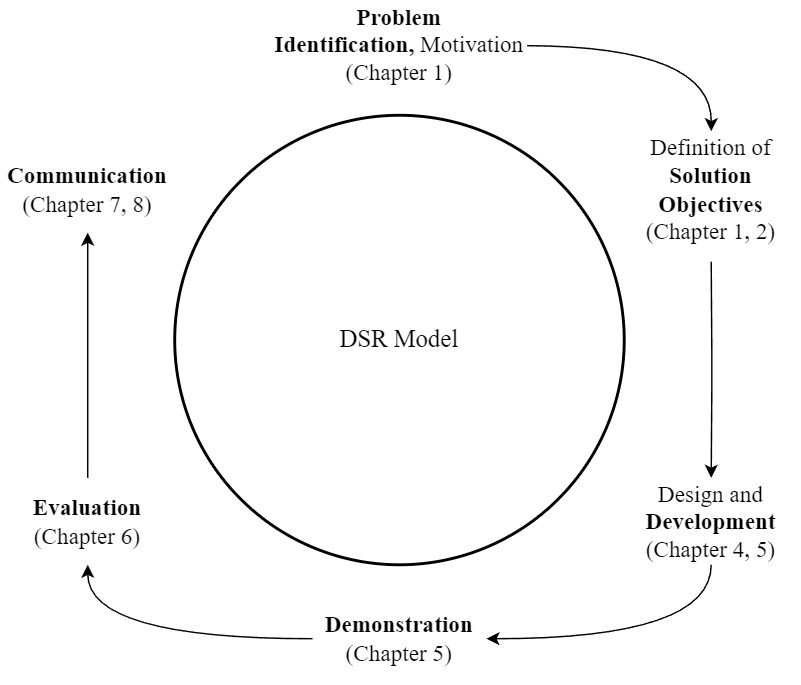
\includegraphics[width=0.8\textwidth]{figures/dsr.png}
  \caption{The cyclical design science research model. The model consists of six steps. The problem identification (1) refers to the research gap in automated VVUQ of SBDT. Defining the solution objectives (2) specifies the research gap by formulating questions and hypotheses based on the theoretical foundations. The design and development (3) phase includes the development of the framework. The demonstration (4) phase shows the application of the framework in a case study. The evaluation (5) phase assesses the effectiveness of the framework. The communication (6) phase concludes the research by presenting the results.}
  \label{fig:DSR}
\end{figure}

The research paradigm of the thesis can be characterized as deductive-theory critical \parencite{eberhard1987einfuhrung}. A conceptual VVUQ framework is developed based on existing theoretical foundations, while deriving new requirements thorugh a requirements analysis. The framework is then applied in a case study to evaluate its effectiveness. The research is critical in the sense that it aims to improve the efficiency and effectiveness of VVUQ for automatically generated DTs. Elements of empirical research are included through the case study and the data-driven approach.

